\documentclass[8pt]{beamer}

\usetheme{metropolis}

\usepackage{emoji}
\usepackage{soul}

\usetikzlibrary{arrows.meta}
\usetikzlibrary{calc}

\title{How evolution gave us free will}
\subtitle{Or did it?}
\author{Esten H. Leonardsen}
\date{01.03.24}

\begin{document}
	\begin{frame}
	 	\titlepage
	\end{frame}

	\begin{frame}{Overview}
		\begin{enumerate}
			\item What is free will and why should we discuss it
			\item Theories of free will
			\item Empirical foundation
			\item Main arguments of the author
			\item Bonus: Why you should believe in free will (even though it doesn't exist)
		\end{enumerate}
	\end{frame}

	\begin{frame}{Background}
		\centering
		\begin{tikzpicture}
			\node[draw=black, inner sep=0pt] at (0, 0) {
				
\includegraphics[width=4cm]{data/book.jpeg}
			};
		\end{tikzpicture}
	\end{frame}

	\begin{frame}{Background: What is free will?}
		\def\linethickness{5pt}
		\def\linecolor{gray}
		\centering
		\begin{tikzpicture}
			\onslide<2->{
				\node[] at (0, 2.2) {Future};
				%\draw[line width=\linethickness, \linecolor!40] (0, -1) -- (0, 2);
				\node[] at (0, -1.2) {Past};
				\only<2>{
					\draw[line width=\linethickness, \linecolor,-stealth] (0, -1) -- (0, 2);
				}
			}

			\onslide<4->{
				\draw[line width=\linethickness, \linecolor!40, -stealth] (0, 0) to [in=270, out=90] (1, 2);
				\draw[line width=\linethickness, \linecolor!40, -stealth] (0, 0) to [in=270, out=90] (2, 2);
				\draw[line width=\linethickness, \linecolor!40, -stealth] (0, 0) to [in=270, out=90] (-1, 2);
				\draw[line width=\linethickness, \linecolor!40, -stealth] (0, 0) to [in=270, out=90] (-2, 2);
			}

			\only<5>{
				\draw[line width=\linethickness, \linecolor!40,-stealth] (0, 0) -- (0, 2);
				\draw[line width=\linethickness, \linecolor, -stealth] (0, 0) to [in=270, out=90] (-1, 2);
			}

			\onslide<3->{
				\draw[line width=\linethickness, \linecolor] (0, -1) -- (0, 0);
				\only<3-4>{
					\draw[line width=\linethickness, \linecolor!40,-stealth] (0, 0) -- (0, 2);
				}
				\node[circle, draw=black, fill=red!60, minimum size=10pt] at (0, 0) {};
				%\draw[line width=\linethickness, \linecolor, -stealth] (0, 0) to [in=270, out=90] (0, 2);
			}


		\end{tikzpicture}
	\end{frame}

	\begin{frame}{Background: Why discuss free will}
		Why is it interesting to discuss whether we have free will?
		\begin{itemize}
			\item To understand what kind of creatures we are and the world we live in.
			\only<1>{
				\item To make moral and just decisions about accountability.
			}
			\only<2>{
				\item[\textcolor{red}{\textbullet}] \textcolor{red}{\st{To make moral and just decisions about accountability.}}
			}
		\end{itemize}
	\end{frame}

	\section{Theories of free will}

	\begin{frame}[c]{Theories of free will}
		\vspace{0.5cm}
		\def\nodesize{2pt}
		\def\nodecolour{blue!60}
		\def\arrowlength{0.3}
		\def\arrowwidth{0.8}

		\centering
		\begin{tikzpicture}
			\node[] at (-2, 2) {};
			\node[] at (7, 2) {};
			\node[] at (2.5, -6) {};

			\only<1-2>{
				\node[] at (2.5, -2) {
					\textbf{Incompatibilism: Free will is incompatible with determinism.}
				};
			}

			\onslide<2->{
				\node (hd) at (0, 0) {
					\only<2->{Hard determinism}
				};
				\node (lfw) at (5, 0) {
					\only<2->{Libertarian free will}
				};
				\draw[<->] (hd) -- (lfw);
			}

			\only<3-5>{
				\draw (-1.5, -5.5) -- (6.5, -5.5) -- (6.5, -2.5) -- (-1.5, -2.5) -- (-1.5, -5.5);
				\node[circle, minimum size=\nodesize, fill=\nodecolour, outer sep=0pt] (n0) at (3.5, -3.5) {};
				\node[circle, minimum size=\nodesize, fill=\nodecolour] (n1) at (0.5, -3) {};
				\node[circle, minimum size=\nodesize, fill=\nodecolour] (n2) at (1.5, -4.5) {};
				\node[circle, minimum size=\nodesize, fill=\nodecolour] (n3) at (4.5, -5) {};
				\node[circle, minimum size=\nodesize, fill=\nodecolour] (n4) at (5.5, -2.9) {};
				\node[circle, minimum size=\nodesize, fill=\nodecolour] (n5) at (0, -4.75) {};

				\only<5>{
					\draw[-stealth, line width=\arrowwidth, draw=\nodecolour] ($ (n0) - (\arrowlength, \arrowlength) $) -- (n0);
				}
				\only<4,5>{
					\draw[-stealth, line width=\arrowwidth, draw=\nodecolour] (n0) -- ($ (n0) + (\arrowlength, \arrowlength) $);
				}

				\only<5>{
					\draw[-stealth, line width=\arrowwidth, draw=\nodecolour] ($ (n1) + (\arrowlength, \arrowlength) $) -- (n1);
				}
				\only<4,5>{
					\draw[-stealth, line width=\arrowwidth, draw=\nodecolour] (n1) -- ($ (n1) - (\arrowlength, \arrowlength) $);
				}
				\only<5>{
					\draw[-stealth, line width=\arrowwidth, draw=\nodecolour] ($ (n2) + (\arrowlength*1.5, \arrowlength/1.5) $) -- (n2);
				}
				\only<4,5>{
					\draw[-stealth, line width=\arrowwidth, draw=\nodecolour] (n2) -- ($ (n2) - (\arrowlength*1.5, \arrowlength/1.5) $);
				}

				\only<5>{
					\draw[-stealth, line width=\arrowwidth, draw=\nodecolour] ($ (n3) - (\arrowlength*2, \arrowlength/2) $) -- (n3);
				}
				\only<4,5>{
					\draw[-stealth, line width=\arrowwidth, draw=\nodecolour] (n3) -- ($ (n3) + (\arrowlength*2, \arrowlength/2) $);
				}

				\only<5>{
					\draw[-stealth, line width=\arrowwidth, draw=\nodecolour] ($ (n4) + (\arrowlength*3, \arrowlength/3) $) -- (n4);
				}
				\only<4,5>{
					\draw[-stealth, line width=\arrowwidth, draw=\nodecolour] (n4) -- ($ (n4) - (\arrowlength*3, \arrowlength/3) $);
				}
				\only<5>{
					\draw[-stealth, line width=\arrowwidth, draw=\nodecolour] ($ (n5) - (\arrowlength*0.5, \arrowlength/0.5) $) -- (n5);
				}
				\only<4,5>{
					\draw[-stealth, line width=\arrowwidth, draw=\nodecolour] (n5) -- ($ (n5) + (\arrowlength*0.5, \arrowlength/0.5) $);
				}
			}
			\onslide<6->{
				\node[anchor=north, align=left, font=\small] at (hd.south) {
					\textcolor{green}{+ Consistent with science}\\
					\textcolor{red}{- Inconsistent with}\\\textcolor{red}{subjective experience}
				};
			}

			\only<8>{
				\node[] at (2.5, -4) {
					
\includegraphics[width=6cm]{data/ratatouille.jpeg}
				};
			}

			\only<9>{
				\node[] at (2.5, -2.6) {
					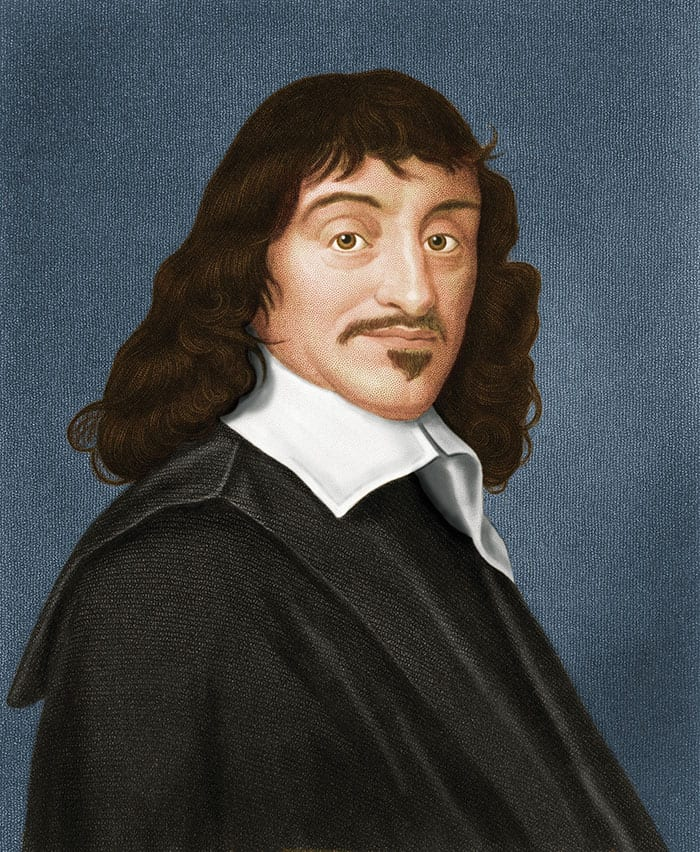
\includegraphics[width=2cm]{data/descartes.jpeg}
				};
				\node[align=center] at (2.5, -4.8) {
					"I have a clear and distinct idea of the mind as a thinking,\\
					non-extended thing. I have a clear and distinct idea of\\
					body as an extended, non-thinking thing. Therefore, the mind\\
					is really distinct from the body and can exist without it."
				};
			}

			\only<10>{
				\node[align=center, inner sep=0pt, draw=black] at (2.5, -4) {
					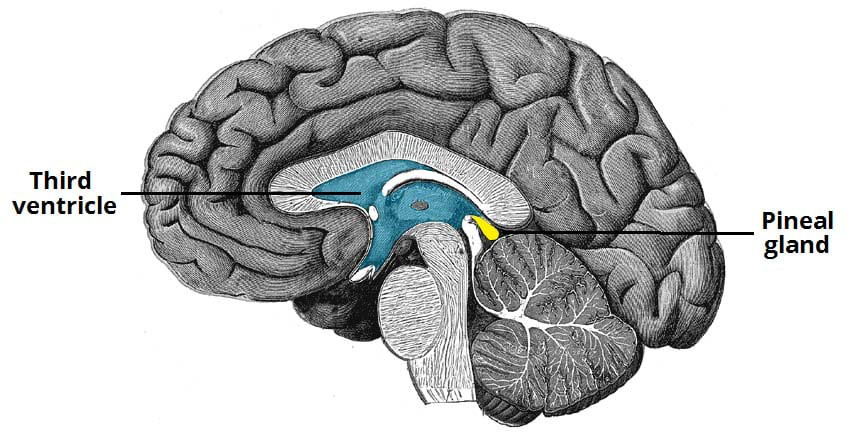
\includegraphics[width=6cm]{data/pineal.jpeg}
				};
			}

			\only<11>{
				\node[align=center] at (2.5, -4) {
					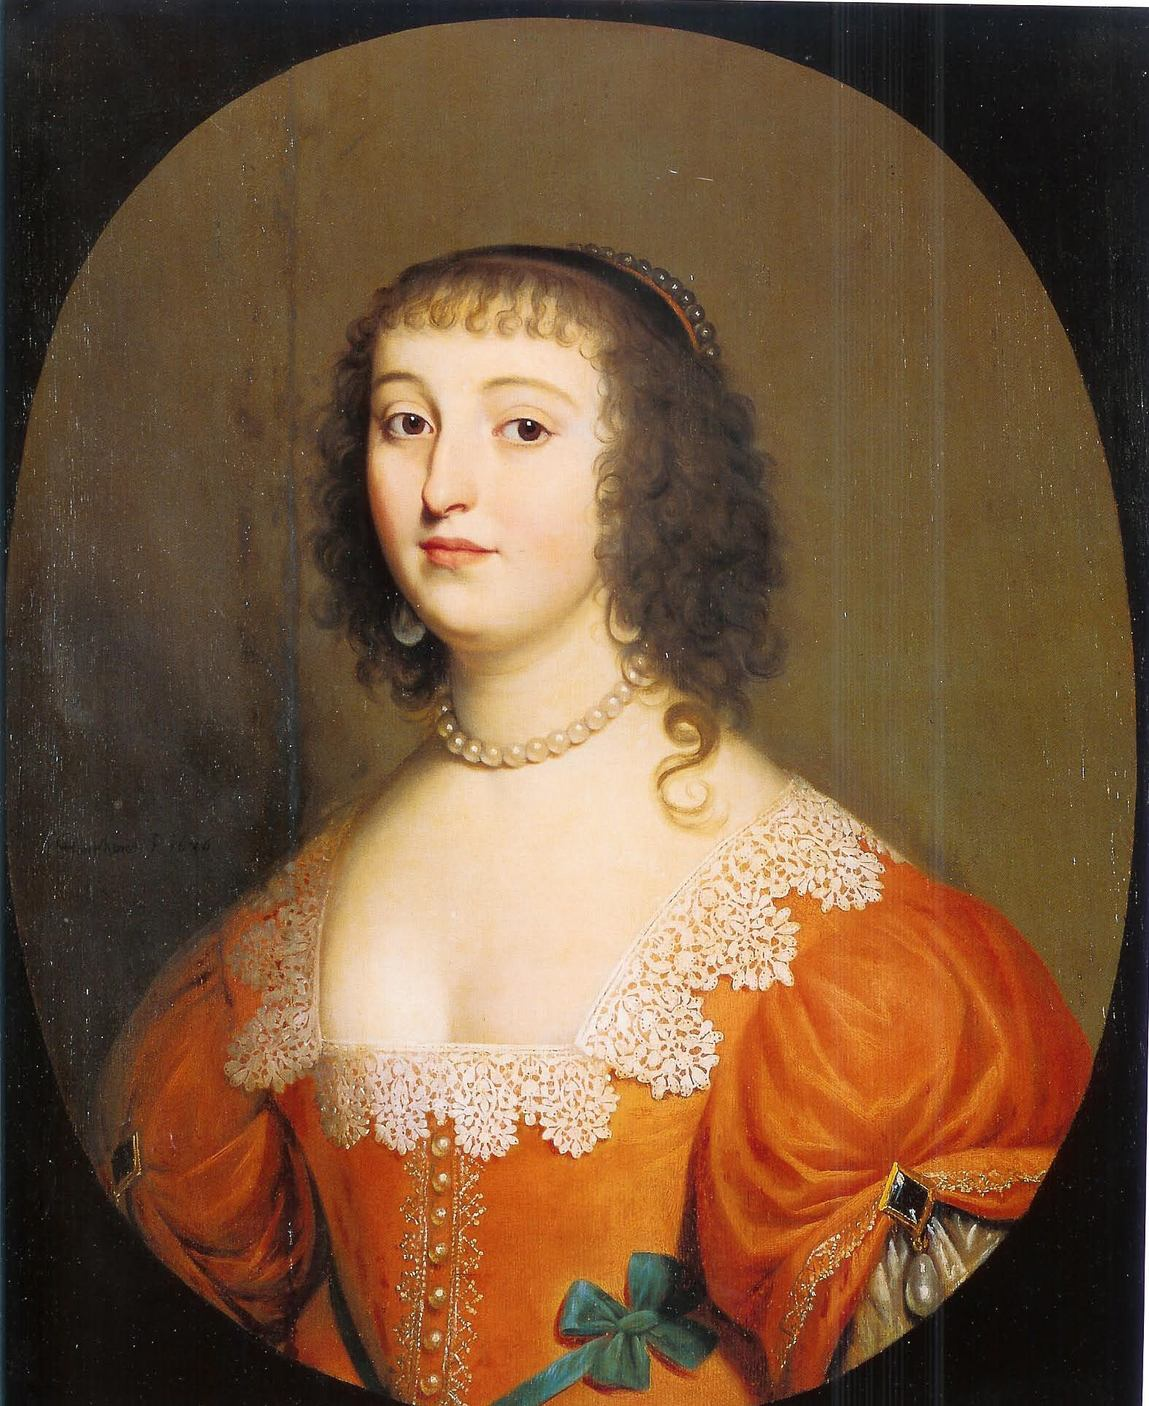
\includegraphics[width=3cm]{data/elisabeth.jpeg}
				};
			}

			\onslide<12->{
				\node[anchor=north, align=left, font=\small] at (lfw.south) {
					\textcolor{green}{+ Consistent with}\\\textcolor{green}{subjective experience}\\
					\textcolor{red}{- Inconsistent with science}
				};
			}

			\only<13>{
				\node[text depth=0] (c) at (2.5, -3) {
					Compatibilism
				};
				\draw[->, dashed] (2.5, 0) -- (c);
			}
		\end{tikzpicture}
	\end{frame}

	\begin{frame}[t]{Theories of free will}
		\textbf{Compatibilism: Determinism and free will are compatible}
		\begin{itemize}
			\onslide<2->{
				\item Dogmatic compatibilism: Free will does not entail freedom of choice.
			}
			\onslide<3->{
				\item Emergentism: Free will emerges from the brain which operates under the laws of physics.
			}
			\onslide<4->{
					\begin{itemize}
					\item Weak emergence: In hierarchical structures, patterns can emerge that appear more meaningful on higher levels of organization.
					\onslide<5->{
						\item Strong emergence: In hierarchical structures, patterns that appear on higher levels can causally influence the levels below them.
					}
				\end{itemize}
			}
		\end{itemize}
		\centering
		\vspace{0.5cm}
		\def\nodesize{2pt}
		\def\nodecolour{blue!60}
		\def\arrowlength{0.3}
		\def\arrowwidth{0.8}
		\onslide<6->{
			\begin{tikzpicture}
				\draw (0, 0) -- (8, 0) -- (8, 3) -- (0, 3) -- (0, 0);
				\node[circle, minimum size=\nodesize, fill=\nodecolour, outer sep=0pt] (n0) at (5, 2) {};
				\node[circle, minimum size=\nodesize, fill=\nodecolour] (n1) at (2, 2.5) {};
				\node[circle, minimum size=\nodesize, fill=\nodecolour] (n2) at (3, 1) {};
				\node[circle, minimum size=\nodesize, fill=\nodecolour] (n3) at (6, 0.5) {};
				\node[circle, minimum size=\nodesize, fill=\nodecolour] (n4) at (7, 2.6) {};
				\node[circle, minimum size=\nodesize, fill=\nodecolour] (n5) at (1.5, 0.75) {};

				\draw[-stealth, line width=\arrowwidth, draw=\nodecolour] ($ (n0) - (\arrowlength, \arrowlength) $) -- (n0);
				\only<6>{
					\draw[-stealth, line width=\arrowwidth, draw=\nodecolour] (n0) -- ($ (n0) + (\arrowlength, \arrowlength) $);
				}
				\onslide<7->{
					\draw[-stealth, line width=\arrowwidth, draw=red] (n0) -- ($ (n0) + (0, 0.5) $);
				}

				\draw[-stealth, line width=\arrowwidth, draw=\nodecolour] ($ (n1) + (\arrowlength, \arrowlength) $) -- (n1);
				\draw[-stealth, line width=\arrowwidth, draw=\nodecolour] (n1) -- ($ (n1) - (\arrowlength, \arrowlength) $);

				\draw[-stealth, line width=\arrowwidth, draw=\nodecolour] ($ (n2) + (\arrowlength*1.5, \arrowlength/1.5) $) -- (n2);
				\draw[-stealth, line width=\arrowwidth, draw=\nodecolour] (n2) -- ($ (n2) - (\arrowlength*1.5, \arrowlength/1.5) $);

				\draw[-stealth, line width=\arrowwidth, draw=\nodecolour] ($ (n3) - (\arrowlength*2, \arrowlength/2) $) -- (n3);
				\draw[-stealth, line width=\arrowwidth, draw=\nodecolour] (n3) -- ($ (n3) + (\arrowlength*2, \arrowlength/2) $);

				\draw[-stealth, line width=\arrowwidth, draw=\nodecolour] ($ (n4) + (\arrowlength*3, \arrowlength/3) $) -- (n4);
				\only<6-7,9->{
					\draw[-stealth, line width=\arrowwidth, draw=\nodecolour] (n4) -- ($ (n4) - (\arrowlength*3, \arrowlength/3) $);
				}
				\only<8>{
					\draw[-stealth, line width=\arrowwidth, draw=red] (n4) -- ($ (n4) - (\arrowlength*3, 0.4) $);
				}
				\draw[-stealth, line width=\arrowwidth, draw=\nodecolour] ($ (n5) - (\arrowlength*0.5, \arrowlength/0.5) $) -- (n5);
				\draw[-stealth, line width=\arrowwidth, draw=\nodecolour] (n5) -- ($ (n5) + (\arrowlength*0.5, \arrowlength/0.5) $);

				\only<10>{
					\node[anchor=east, inner sep=0pt] at (8, 1.8) {
						
\includegraphics[width=3cm]{data/hand_of_god.png}
					};
				}
				%\draw[densely dotted] (8, 1) -- (n0);
			\end{tikzpicture}
		}
	\end{frame}

	\begin{frame}[c]{Theories of free will}
		\centering
		\begin{tikzpicture}
			\node[] at (-2, 2) {};
			\node[] at (7, 2) {};
			\node[] at (2.5, -6) {};

			\node (hd) at (0, 0) {
				Hard determinism
			};
			\node (lfw) at (5, 0) {
				Libertarian free will
			};
			\node[text depth=0] (c) at (2.5, -3) {
				Compatibilism
			};

			\draw[<->] (hd) -- (lfw);
			\draw[->, dashed] (2.5, 0) -- (c);

			\node[anchor=north, align=left, font=\small] at (hd.south) {
				\textcolor{green}{+ Consistent with science}\\
				\textcolor{red}{- Inconsistent with}\\\textcolor{red}{subjective experience}
			};

			\node[anchor=north, align=left, font=\small] at (lfw.south) {
				\textcolor{green}{+ Consistent with}\\\textcolor{green}{subjective experience}\\
				\textcolor{red}{- Inconsistent with science}
			};

			\node[anchor=north, align=left, font=\small] at (c.south) {
				\textcolor{green}{+ Anything goes}\\
				\textcolor{red}{- Anything goes}
			};
		\end{tikzpicture}
	\end{frame}

	\section{Empirical foundation}

	\begin{frame}{Empirical foundation: Libet experiments}
		\centering
		"The onset of cerebral activity clearly preceded by at least several hundred milliseconds the reported time of conscious intention to act."

		\vspace{0.5cm}

		\textit{TIME OF CONSCIOUS INTENTION TO ACT
		IN RELATION TO ONSET OF CEREBRAL
		ACTIVITY (READINESS-POTENTIAL), Libet et al. (1983), Brain}

	\end{frame}

	\begin{frame}{Empirical foundation: Libet experiments}
		\centering
		\begin{tikzpicture}
			\node[] at (0, 0) {
				
\includegraphics[width=5cm]{data/libet.png}
			};

			\onslide<2->{
				\draw[] (-3.5, -3.3) -- (3.5, -3.3) -- (3.5, -4.3) -- (-3.5, -4.3) -- cycle;
				\node[anchor=north] at (0, -4.3) {\textit{time}};
			}

			\only<3-9>{
				\draw[densely dotted] (0.4, -3.3) -- (0.4, -4.3);
				\node[anchor=south] at (0.4, -3.3) {\Large{\emoji{light-bulb}}};
			}

			\onslide<4->{
				\draw[densely dotted] (1.2, -3.3) -- (1.2, -4.3);
				\node[anchor=south] at (1.2, -3.3) {\Large{\emoji{backhand-index-pointing-down}}};
			}

			\only<5-6,9->{
				\draw[red] plot [smooth] coordinates {
					(-3.5, -4)
					(0, -4)
					(1, -3.5)
					(2, -4)
					(3.5, -4)
				};
			}

			\onslide<6->{
				\node[anchor=south] at (0, -3.3) {\Large{\emoji{brain}}};
				\draw[densely dotted] (0, -3.3) -- (0, -4.3);
			}

			\onslide<7-8>{
				\draw[red] plot [smooth] coordinates {
					(-3.5, -4)
					(-3, -3.9)
					(-2.7, -4.1)
					(-2.2, -3.85)
					(-1.8, -4)
					(-1, -3.8)
					(0, -4)
					(1, -3.5)
					(2, -4)
					(2.5, -3.9)
					(3.5, -4)
				};
			}

			\only<8>{
				\draw[dashed] (-3.5, -3.78) -- (3.5, -3.78);
			}

			\only<10>{
				\node[anchor=south] at (0.4, -3.3) {\Large{\emoji{eyes}}};
				\draw[densely dotted] (0.4, -3.3) -- (0.4, -4.3);
			}

		\end{tikzpicture}
	\end{frame}

	\begin{frame}{Empirical foundation: Priming}
		\centering
		"It is concluded that social stimuli of which people are not consciously aware can influence conscious judgments."

		\vspace{0.5cm}

		\textit{Automatic information processing and social perception: The influence of trait information presented outside of conscious awareness on impression formation., Bargh et al. (1982), Journal of Personality and Social Psychology}
	\end{frame}

	\begin{frame}{Empirical foundation: Explanations}
	\end{frame}

	\begin{frame}{Empirical foundation: Explanations}
		\centering
		\begin{tikzpicture}
			\node[] (lb) at (0, 0) {
				
\includegraphics[width=1.5cm]{data/brainhalf.png}
			};
			\only<1-6>{
				\node[] (rb) at (1.8, 0) {
					\scalebox{-1}[1]{
\includegraphics[width=1.5cm]{data/brainhalf.png}}
				};
			}

			\onslide<2->{
				\only<2-6>{
					\node[rotate=180, inner sep=0pt] (le) at (0.2, 2) {\Huge{\emoji{eye}}};
				}
				\node[rotate=180, inner sep=0pt] (re) at (1.6, 2) {\Huge{\emoji{eye}}};
			}

			\onslide<3->{
				\only<3-6>{
					\draw[-stealth, line width=3pt, draw=red, opacity=0.5] (le.north) to [in=90, out=270] (rb.center);
				}
				\draw[-stealth, line width=3pt, draw=blue, opacity=0.5] (re.north) to [in=90, out=270] (lb.center);
			}

			\onslide<4->{
				\node[draw=black, inner sep=0pt] at (2.2, 4) {
					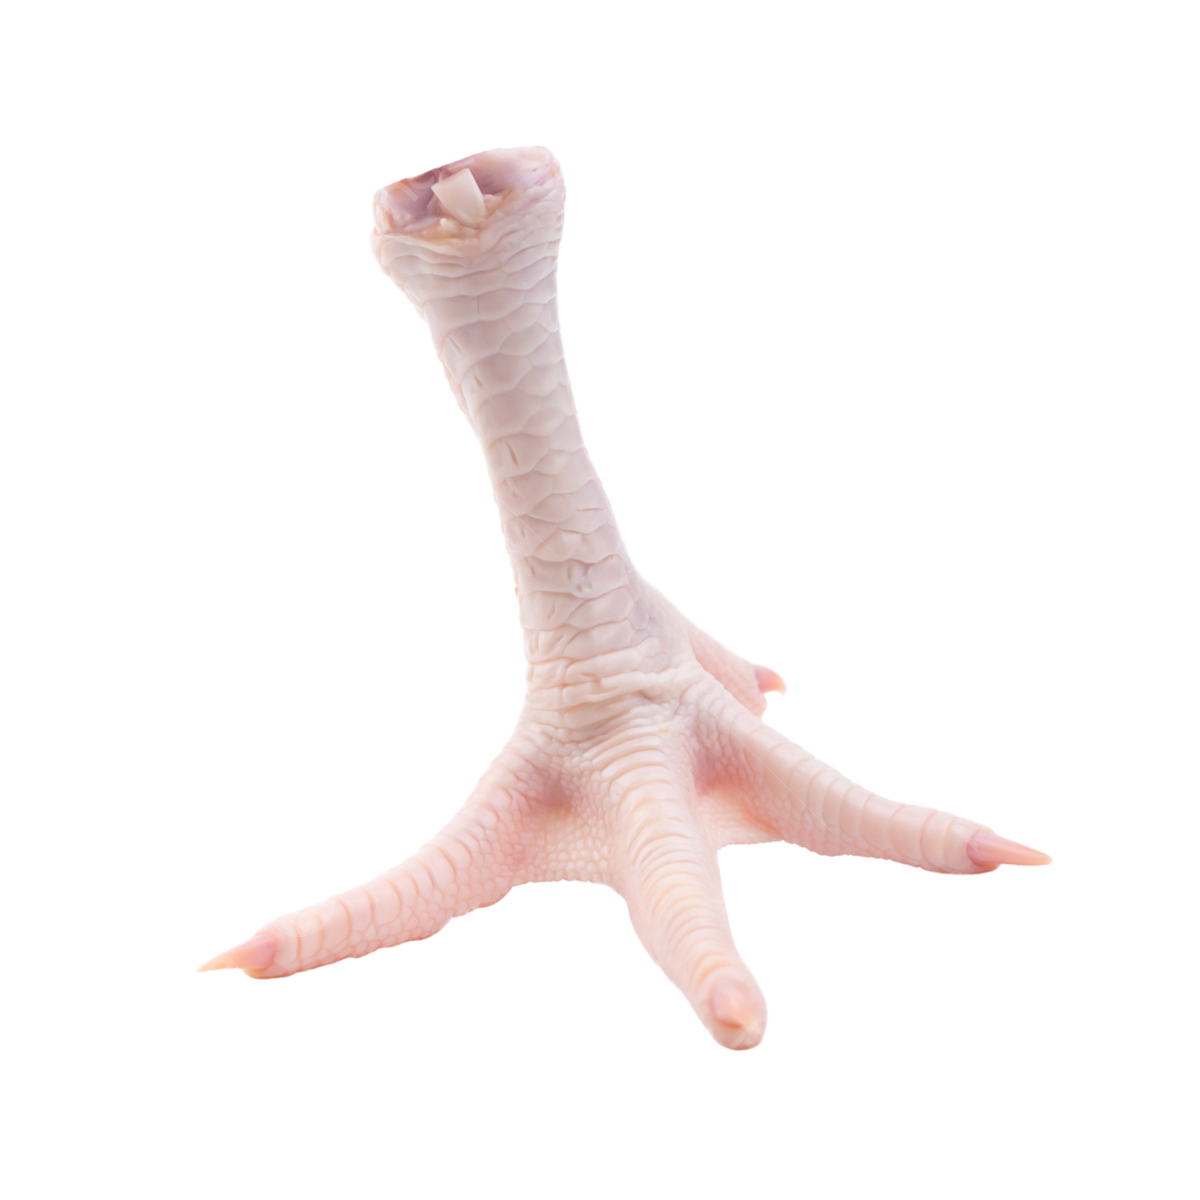
\includegraphics[width=2cm]{data/claw.jpeg}
				};
				\only<4-6>{
					\node[draw=black, inner sep=0pt] at (-0.4, 4) {
						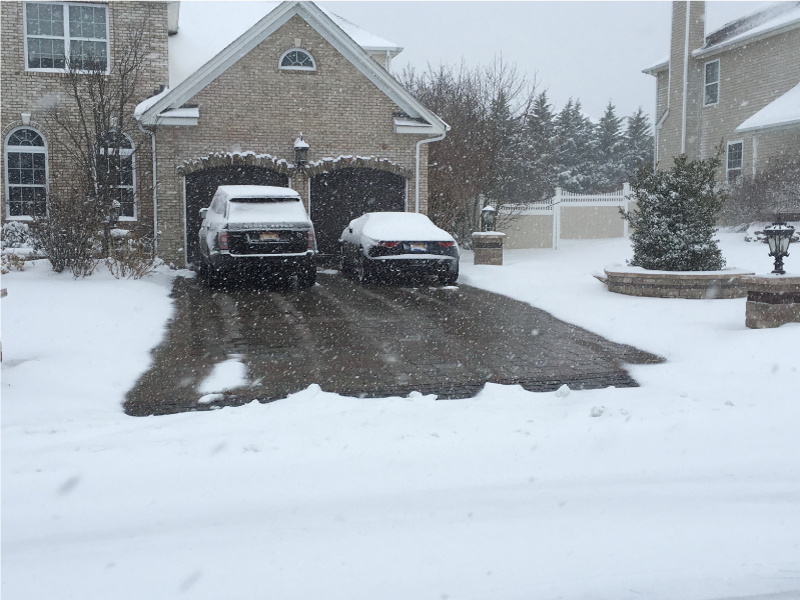
\includegraphics[width=2cm]{data/snow.png}
					};
				}
			}

			\onslide<5->{
				\node[draw=black, inner sep=0pt] (shovel) at (-3, 0) {
					
\includegraphics[width=2cm]{data/shovel.jpeg}
				};
				\node[draw=black, inner sep=0pt] (chicken) at (4.8, 0) {
					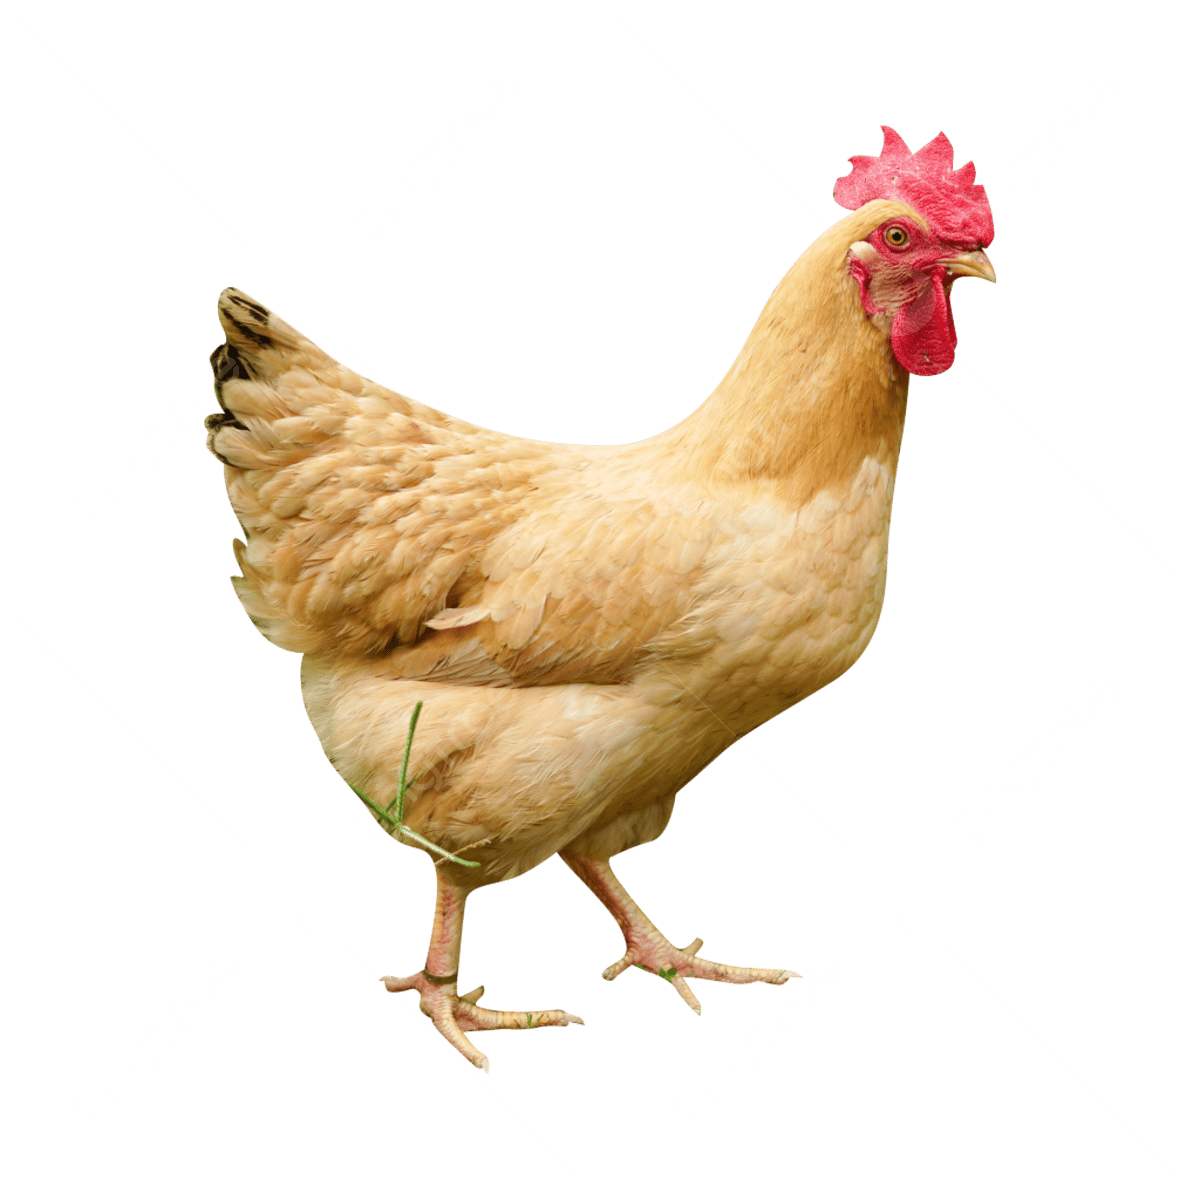
\includegraphics[width=2cm]{data/chicken.png}
				};
				\draw[-stealth, line width=3pt, draw=blue, opacity=0.5] ($ (lb.center) - (0, 1) $) to [in=180, out=0] (chicken);
				\only<5-6>{
					\draw[-stealth, line width=3pt, draw=red, opacity=0.5] ($ (rb.center) - (0, 1) $) to [in=0, out=180] (shovel);
				}
			}

			\only<6-7>{
				\node[fill=orange, opacity=0.5, circle, minimum size=25pt] at (-0.3, 0.2) {};
			}
		\end{tikzpicture}
	\end{frame}

	\begin{frame}{Empirical foundation: Explanations}
		What did the left brain answer when asked why it pointed to a shovel?
		\begin{itemize}
			\item[a.] Because it can be used to shovel snow
			\item[b.] No idea
			\item[c.] Because it can be used to clean the chicken shed
		\end{itemize}
	\end{frame}

	\section{The book}

	\begin{frame}{Argument one}
		\begin{enumerate}
			\item An entity is a being which is shielded from the world.
			\item Being alive means that your inside is more structured than the outside, and you strive to keep it that way.
			\item Movement gives you options to harvest resources from the outside to retain your internal structure.
			\item Sensors gives you the opportunity to move in a targetted manner.
			\item Monitoring your internal states allows you to prioritize outcomes.
			\item A nervous system that connects your sensors (both internal and external) to your moveable parts allows you to choose actions, based on your surroundings and needs.
			\item The strategy that underlies these choices are shaped by evolution (through DNA) and learning (through the nervous system).
			\item[\rightarrow] This is free will!
			\only<2>{\item[\rightarrow] This is dogmatic compatibilism.}
		\end{enumerate}
	\end{frame}

	\begin{frame}{Argument two}
		\centering
		\begin{tikzpicture}
			\node[circle, minimum size=20pt, draw=blue!60, fill=blue!60] (n1) at (0, 0) {};
			\draw[-stealth, draw=blue!60, line width=3pt] (n1) -- ($ (n1) + (1.5, 0) $);
			\onslide<2->{
				\draw[-stealth, draw=blue!60, line width=3pt, opacity=0.25] (n1) -- ($ (n1) + (1.5, 1) $);
				\draw[-stealth, draw=blue!60, line width=3pt, opacity=0.5] (n1) -- ($ (n1) + (1.5, 0.5) $);
				\draw[-stealth, draw=blue!60, line width=3pt, opacity=0.5] (n1) -- ($ (n1) + (1.5, -0.5) $);
				\draw[-stealth, draw=blue!60, line width=3pt, opacity=0.25] (n1) -- ($ (n1) + (1.5, -1) $);
			}
			\draw[-stealth, draw=blue!60, line width=3pt] ($ (n1) - (1.5, 0) $) -- (n1);

			\onslide<3->{
				\node[circle, minimum size=20pt, draw=red!60, fill=red!60] (n1) at (0, -2.5) {};
				\draw[-stealth, draw=red!60, line width=3pt, opacity=0.25] (n1) -- ($ (n1) + (1.5, 0) $);

				\draw[-stealth, draw=red!60, line width=3pt] (n1) -- ($ (n1) + (1.5, 1) $);
				\draw[-stealth, draw=red!60, line width=3pt, opacity=0.5] (n1) -- ($ (n1) + (1.5, 0.5) $);
				\draw[-stealth, draw=red!60, line width=3pt, opacity=0.125] (n1) -- ($ (n1) + (1.5, -0.5) $);
				\draw[-stealth, draw=red!60, line width=3pt, opacity=0.0675] (n1) -- ($ (n1) + (1.5, -1) $);

				\draw[-stealth, draw=red!60, line width=3pt] ($ (n1) - (1.5, 0) $) -- (n1);
			}
		\end{tikzpicture}
	\end{frame}

	\begin{frame}{Argument two}
		\begin{itemize}
			\item The low-level details of a nervous system and the laws of physics do not fully explain how a system evolves nor behaves.
			\item This lee-way allows agents to choose between equally probable next states.
			\item[\rightarrow] This is free will!
			\only<2>{\item[\rightarrow] This is strong emergentism}
		\end{itemize}
	\end{frame}

	\section{My argument}

	\begin{frame}{My argument}
		\centering
		\begin{tikzpicture}
			\draw[] (0, 0) -- (3, 0);
			\draw[] (3, 0) -- (3, 3);
			\draw[] (3, 3) -- (0, 3);
			\draw[] (0, 3) -- (0, 0);
			\draw[] (1.5, 0) -- (1.5, 3);

			\node[anchor=south] at (1.5, 3.5) {Free will exists};
			\node[anchor=south] at (0.75, 3) {Yes};
			\node[anchor=south] at (2.25, 3) {No};

			\onslide<2->{
				\draw[] (0, 1.5) -- (3, 1.5);
				\node[anchor=south, rotate=90] at (-0.5, 1.5) {We believe in free will};
				\node[anchor=south, rotate=90] at (0, 0.75) {No};
				\node[anchor=south, rotate=90] at (0, 2.25) {Yes};
			}
			\onslide<3->{
				\node[] at (0.75, 2.25) {$n_{0,0}$};
				\node[] at (2.25, 2.25) {$n_{0,1}$};
				\node[] at (0.75, 0.75) {$n_{1,0}$};
				\node[] at (2.25, 0.75) {$n_{1,1}$};
			}

			\onslide<5->{
				\draw[orange, thick, fill=orange, fill opacity=0.25] (0, 0) -- (3, 0) -- (3, 1.5) -- (0, 1.5) -- cycle;
				\draw[purple, thick, fill=purple, fill opacity=0.25] (0, 1.5) -- (3, 1.5) -- (3, 3) -- (0, 3) -- cycle;
			}

			% n00
			\only<7-9,11>{
				\draw[white, fill=white, opacity=0.75] (0, 1.5) -- (1.5, 1.5) -- (1.5, 3) -- (0, 3) -- cycle;
			}
			% n01
			\only<4,6,8-9,12>{
				\draw[white, fill=white, opacity=0.75] (1.5, 1.5) -- (3, 1.5) -- (3, 3) -- (1.5, 3) -- cycle;
			}
			% n10
			\only<4,6-7,9,11>{
				\draw[white, fill=white, opacity=0.75] (0, 0) -- (1.5, 0) -- (1.5, 1.5) -- (0, 1.5) -- cycle;
			}
			% n11
			\only<6-8,12>{
				\draw[white, fill=white, opacity=0.75] (1.5, 0) -- (3, 0) -- (3, 1.5) -- (1.5, 1.5) -- cycle;
			}

			\only<6-12>{
				\node[anchor=west] at (-2.25, -1) {
					\only<6>{
						\textcolor{purple}{$p_f * n_{0,0}$}
					}
					\only<7>{
						\textcolor{purple}{$p_f * n_{0,0} - (1 - p_f) * n_{0,1}$}
					}
					\only<8>{
						\textcolor{purple}{$p_f * n_{0,0} - (1 - p_f) * n_{0,1}$} > \textcolor{orange}{$p_f * n_{1,0}$}
					}
					\only<9-11>{
						\textcolor{purple}{$p_f * n_{0,0} - (1 - p_f) * n_{0,1}$} > \textcolor{orange}{$p_f * n_{1,0} - (1 - p_f) * n_{1,1}$}
					}
					\only<12>{
						\textcolor{purple}{$p_f * n_{0,0}$}\textcolor{purple!20}{$ - (1 - p_f) * n_{0,1}$} > \textcolor{orange}{$p_f * n_{1,0}$}\textcolor{orange!20}{$ - (1 - p_f) * n_{1,1}$}
					}
				};
			}

			\node[] at (-2.5, 5) {};
			\node[] at (5.5, -3) {};
		\end{tikzpicture}
	\end{frame}

	\begin{frame}{My argument}
		\centering
		\begin{tikzpicture}
			\node[] at (0, 0) {
				
\includegraphics[width=9cm]{data/moxness.png}
			};
			\node[rotate=30] at (-4.2, 2.5) {\textbf{\Huge{Stem rødt!}}};
			\node[rotate=-15] at (1, -1) {\textbf{\Huge{\textcolor{white}{Foxy Moxy på tinget!}}}};
		\end{tikzpicture}
	\end{frame}

	\begin{frame}[t]{Summary}
		\begin{itemize}
			\item Free will doesn't exist
			\onslide<2->{\item But you should pretend it does!}
			\onslide<3->{\item But not too much!!}
		\end{itemize}

		\vspace{5cm}

		\centering
		\only<4>{\textbf{Thank you for coming to my TED-talk!}}
	\end{frame}


\end{document}
